\documentclass[10pt]{article}
\usepackage[T1]{fontenc}
\usepackage[utf8]{inputenc}
\usepackage{lmodern}
\usepackage[a4paper,margin=1in]{geometry}
\usepackage{amsmath,amssymb,amsthm,mathtools,bm}
\usepackage{graphicx}
\usepackage{booktabs}
\usepackage{enumitem}
\usepackage{xcolor}
\usepackage{caption}
\usepackage{subcaption}
\usepackage{hyperref}
\usepackage[nameinlink,capitalise,noabbrev]{cleveref}
\usepackage{float}
\usepackage{setspace}
\usepackage{fancyhdr}
\usepackage{array}
\usepackage{multirow}
\usepackage{longtable}
\usepackage{tikz}
\usepackage{microtype}

\setstretch{1.08}
\setlength{\parskip}{0.45em}
\setlength{\parindent}{0pt}
\setlength{\headheight}{14pt}
\allowdisplaybreaks
\numberwithin{equation}{section}

\pagestyle{fancy}
\fancyhf{}
\fancyhead[L]{Diffusion on AR(1) sequences}
\fancyhead[R]{\thepage}
\renewcommand{\headrulewidth}{0.4pt}

\newtheorem{theorem}{Theorem}[section]
\newtheorem{proposition}[theorem]{Proposition}
\newtheorem{lemma}[theorem]{Lemma}
\newtheorem{corollary}[theorem]{Corollary}
\theoremstyle{definition}
\newtheorem{definition}[theorem]{Definition}
\newtheorem{example}[theorem]{Example}
\theoremstyle{remark}
\newtheorem{remark}[theorem]{Remark}

\newcommand{\R}{\mathbb{R}}
\newcommand{\E}{\mathbb{E}}
\newcommand{\Var}{\operatorname{Var}}
\newcommand{\Cov}{\operatorname{Cov}}
\newcommand{\diag}{\operatorname{diag}}
\newcommand{\Id}{I}
\newcommand{\trans}{\mathsf{T}}
\newcommand{\diff}{\,\mathrm{d}}
\newcommand{\Ncal}{\mathcal{N}}
\newcommand{\norm}[1]{\lVert #1\rVert}
\newcommand{\inner}[2]{\langle #1,#2\rangle}
\newcommand{\argmax}{\operatorname*{arg\,max}}
\newcommand{\argmin}{\operatorname*{arg\,min}}
\newcommand{\Corr}{\operatorname{Corr}}
\newcommand{\tr}{\operatorname{tr}}
\newcommand{\sgn}{\operatorname{sgn}}

\geometry{a4paper,margin=0.85in}
\setstretch{1.03}
\setlength{\parskip}{0.35em}

\hypersetup{
  colorlinks=true,
  linkcolor=blue!55!black,
  citecolor=blue!55!black,
  urlcolor=blue!55!black,
  pdftitle={Short presentation note on diffusion over correlated sequences},
  pdfauthor={OpenAI synthesis manuscript}
}

\title{\textbf{Short Presentation Note:}\\
Markov Locality, Diffusion Fill-In, and the First Non-Gaussian Route}
\author{Compact note aligned with the current manuscript}
\date{March 2026}

\begin{document}
\maketitle
\thispagestyle{empty}

\begin{abstract}
The Gaussian AR(1) benchmark is solved. What remains is to understand the structural question behind it: how the local Markov geometry of the clean chain appears in the score, how diffusion reshapes that locality at intermediate times, and how isotropic noise eventually erases it. This short note extracts the strongest benchmark facts, the deterministic control experiment, the first non-Gaussian extension, and the observables that should organize the next stage of the project.
\end{abstract}

\section{Benchmark and open problem}

The solved Gaussian benchmark is
\begin{equation}
 a_{k+1}=\alpha a_k+\eta_k,
 \qquad |\alpha|<1,
 \qquad \eta_k\sim\Ncal(0,\sigma_\eta^2),
\end{equation}
observed through coordinate-wise OU noising,
\begin{equation}
 x_k=e^{-t}a_k+\sqrt{\Delta_t}\,z_k,
 \qquad \Delta_t=1-e^{-2t}.
\end{equation}
The key formulas are
\begin{equation}
 \Sigma_t=e^{-2t}\Sigma_0+\Delta_t\Id,
 \qquad
 S(\mathbf x,t)=\nabla\log p_t(\mathbf x)=-Q_t(\mathbf x-\boldsymbol\mu_t),
 \qquad Q_t=\Sigma_t^{-1}.
\end{equation}
The benchmark cleanly separates two ingredients:
\begin{itemize}[leftmargin=1.1cm]
\item \textbf{Gaussianity:} the score is affine and the eigenbasis of $\Sigma_0$ diagonalizes the whole problem.
\item \textbf{Markovianity:} the clean precision $Q_0$ is tridiagonal because the path measure is built from nearest-neighbor transition factors.
\end{itemize}
The next question is therefore:
\begin{quote}
\emph{How does the local Markov structure survive, deform, and disappear in the score under diffusion?}
\end{quote}

\section{Gaussian benchmark: the precision lifecycle}

At clean time,
\begin{equation}
 p_0(\mathbf a)
 \propto
 \exp\!\left[-\frac{(a_0-\mu_0)^2}{2\sigma_0^2}
 -\frac{1}{2\sigma_\eta^2}\sum_{k=0}^{K-1}(a_{k+1}-\alpha a_k)^2\right],
\end{equation}
so $Q_0$ is tridiagonal. This is the algebraic expression of the Markov property: after conditioning on all other frames, each frame interacts only with its nearest neighbors.

The covariance and precision react very differently to diffusion:
\begin{equation}
 (\Sigma_t)_{jk}=e^{-2t}(\Sigma_0)_{jk}
 \qquad (j\neq k),
\end{equation}
so the covariance keeps the same off-diagonal profile and only contracts. By contrast,
\begin{equation}
 Q_t=U\diag\!\left(\frac{1}{e^{-2t}\lambda_i+\Delta_t}\right)U^\top
 =\frac{1}{\Delta_t}(\Id+\gamma_t\Sigma_0)^{-1},
 \qquad \gamma_t=\frac{e^{-2t}}{\Delta_t},
\end{equation}
which generically destroys the delicate spectral cancellations that made $Q_0$ tridiagonal.

The small-time expansion is the cleanest statement of immediate fill-in:
\begin{equation}
 Q_t=e^{2t}\sum_{m\geq 0}(-c_t)^mQ_0^{m+1},
 \qquad c_t=e^{2t}-1.
\end{equation}
If $|i-j|=d\geq 2$, then
\begin{equation}
 (Q_t)_{ij}=(-1)^{d-1}(2t)^{d-1}(Q_0^d)_{ij}+O(t^d).
\end{equation}
Therefore distance-$d$ couplings appear at order $t^{d-1}$: the matrix becomes exact-full for arbitrarily small $t>0$, but farther couplings are initially tiny. At large time,
\begin{equation}
 Q_t=\Id-e^{-2t}(\Sigma_0-\Id)+O(e^{-4t}),
\end{equation}
so all off-diagonal entries vanish exponentially and the score becomes entrywise independent.

\begin{figure}[H]
\centering

\includegraphics[width=.92\textwidth]{figures/fig01_sigma0_vs_precision0.pdf}
\caption{Dense clean covariance versus tridiagonal clean precision. Covariance measures marginal propagation; precision measures direct conditional dependence.}
\end{figure}

\begin{figure}[H]
\centering

\includegraphics[width=.98\textwidth]{figures/fig02_sigma_t_panel.pdf}
\caption{Lifecycle of the covariance and precision. The precision follows the structural path tridiagonal $\to$ full $\to$ diagonal.}
\end{figure}

\begin{figure}[H]
\centering
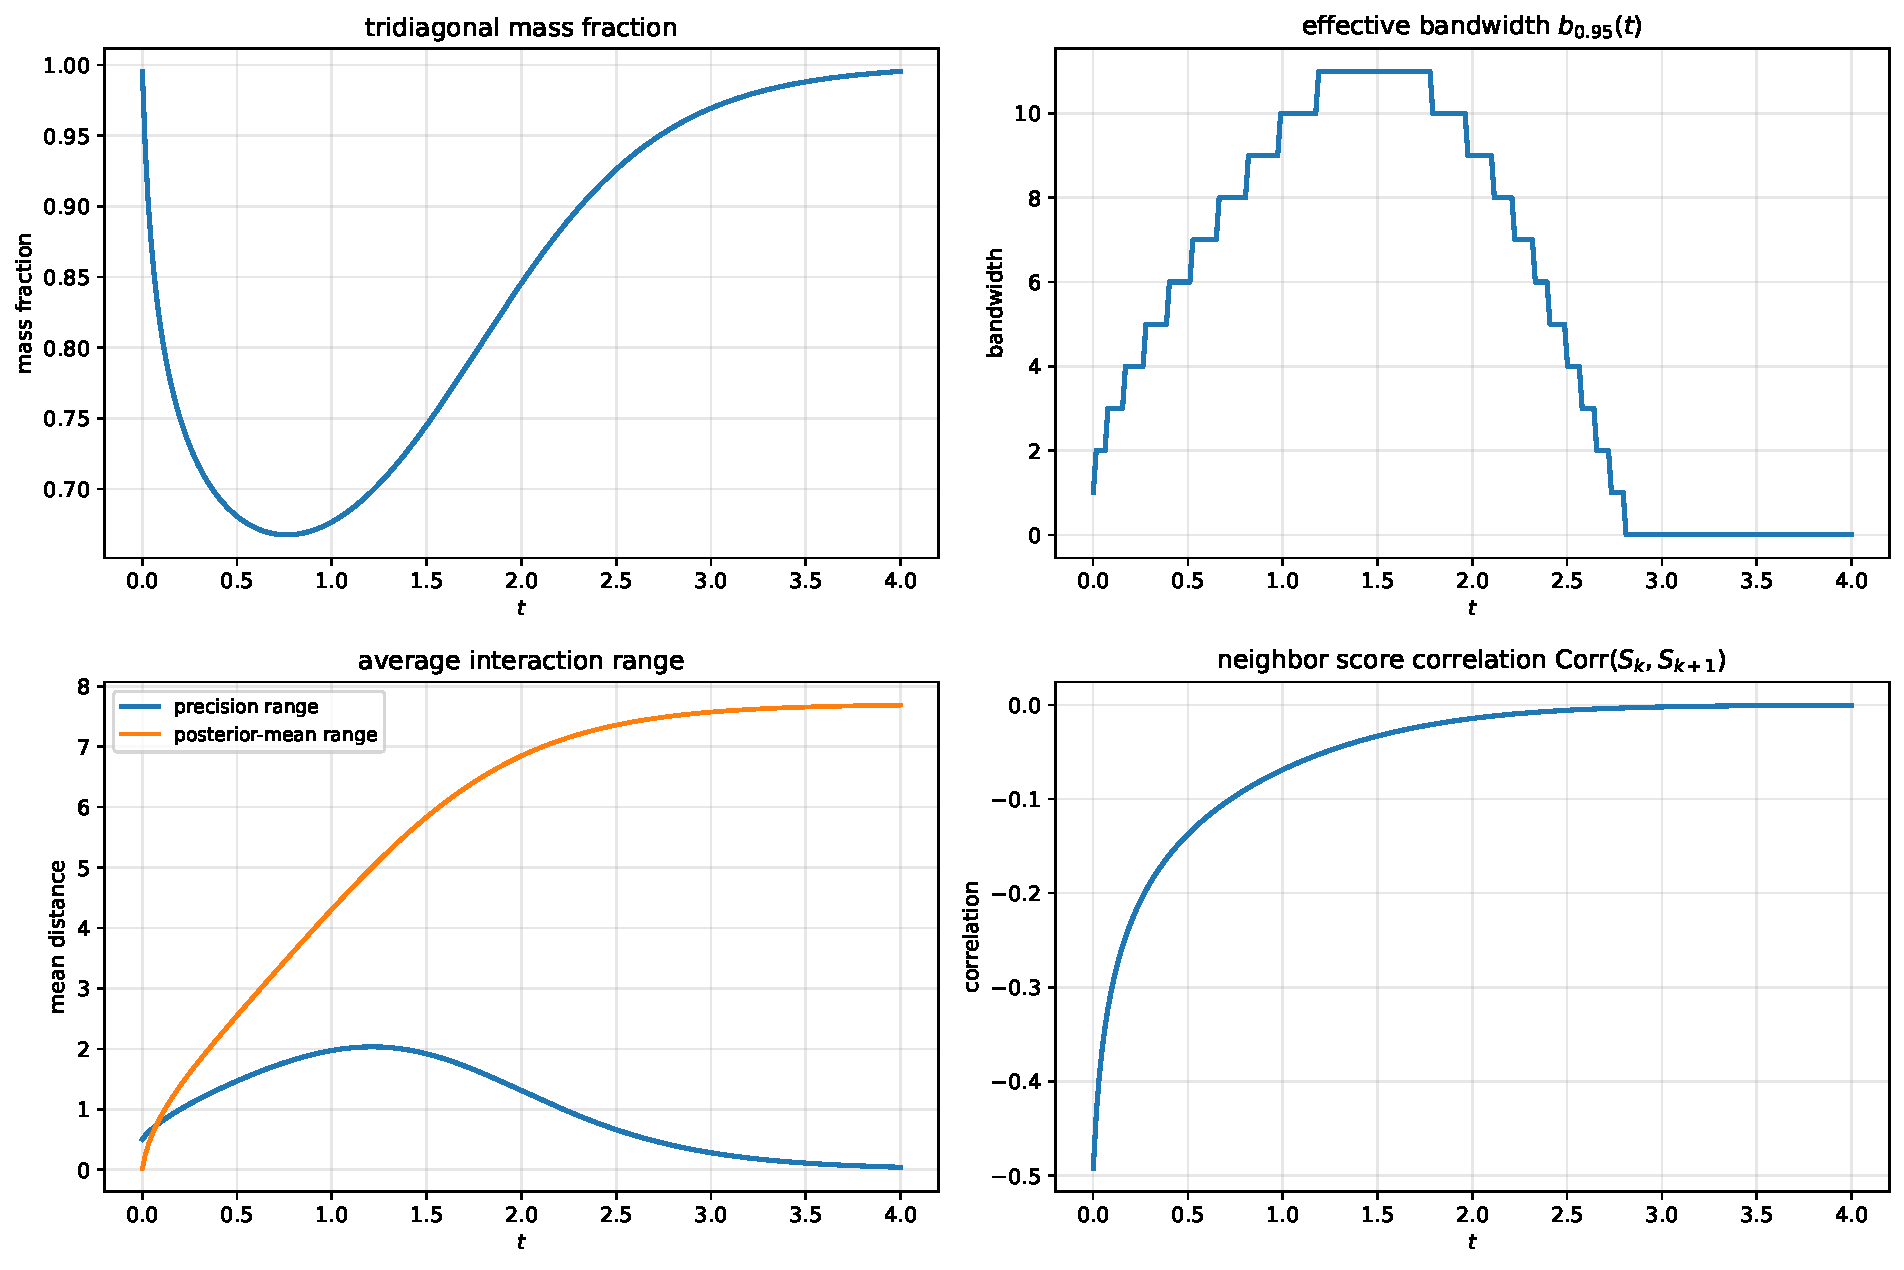
\includegraphics[width=.92\textwidth]{figures/fig10_locality_observables.pdf}
\caption{Locality observables versus diffusion time: tridiagonal mass fraction, effective bandwidth, average interaction range, and neighboring-score correlation.}
\end{figure}

\section{Two extra viewpoints requested in the meeting}

\subsection*{Neighboring score components}
Because $S_t=-Q_t(\mathbf X_t-\boldsymbol\mu_t)$ and $\mathbf X_t\sim\Ncal(\boldsymbol\mu_t,\Sigma_t)$,
\begin{equation}
 \Cov(S_t)=Q_t.
\end{equation}
So in the Gaussian benchmark the relation between $S_k$ and $S_{k+1}$ is encoded exactly by $(Q_t)_{k,k+1}$ and its normalized version
\begin{equation}
 \Corr(S_k,S_{k+1})=\frac{(Q_t)_{k,k+1}}{\sqrt{(Q_t)_{kk}(Q_t)_{k+1,k+1}}}.
\end{equation}

\subsection*{Posterior mean viewpoint}
The vector Tweedie formula gives
\begin{equation}
 \E[\mathbf a\mid \mathbf X_t=\mathbf x]=e^t\big(\mathbf x+\Delta_tS(\mathbf x,t)\big).
\end{equation}
In the Gaussian benchmark,
\begin{equation}
 \E[\mathbf a\mid \mathbf X_t=\mathbf x]
 =\boldsymbol\mu_0+G_t(\mathbf x-\boldsymbol\mu_t),
 \qquad G_t=e^{-t}\Sigma_0Q_t.
\end{equation}
The matrix $G_t$ is the posterior-mean gain. It often gives a more intuitive reconstruction-based notion of locality than the score itself.

\section{Deterministic control experiment}

To isolate what comes from propagation alone, set the innovation noise to zero and keep only a random initial condition:
\begin{equation}
 a_k=\alpha^kA_0,
 \qquad A_0\sim\Ncal(\mu_0,\sigma_0^2).
\end{equation}
Then
\begin{equation}
 \Sigma_0^{\mathrm{det}}=\sigma_0^2vv^\top,
 \qquad v=(1,\alpha,\dots,\alpha^K)^\top,
\end{equation}
which is rank one. After OU noising,
\begin{equation}
 \Sigma_t^{\mathrm{det}}=e^{-2t}\sigma_0^2vv^\top+\Delta_t\Id,
\end{equation}
with exact inverse
\begin{equation}
 Q_t^{\mathrm{det}}=\frac{1}{\Delta_t}\Id-
 \frac{e^{-2t}\sigma_0^2}{\Delta_t^2\left(1+\frac{e^{-2t}\sigma_0^2}{\Delta_t}\|v\|^2\right)}vv^\top.
\end{equation}
Hence every off-diagonal entry is generically nonzero for every $t>0$. This shows that global couplings can arise from deterministic propagation of a single latent amplitude, even without innovation randomness.

\begin{figure}[H]
\centering
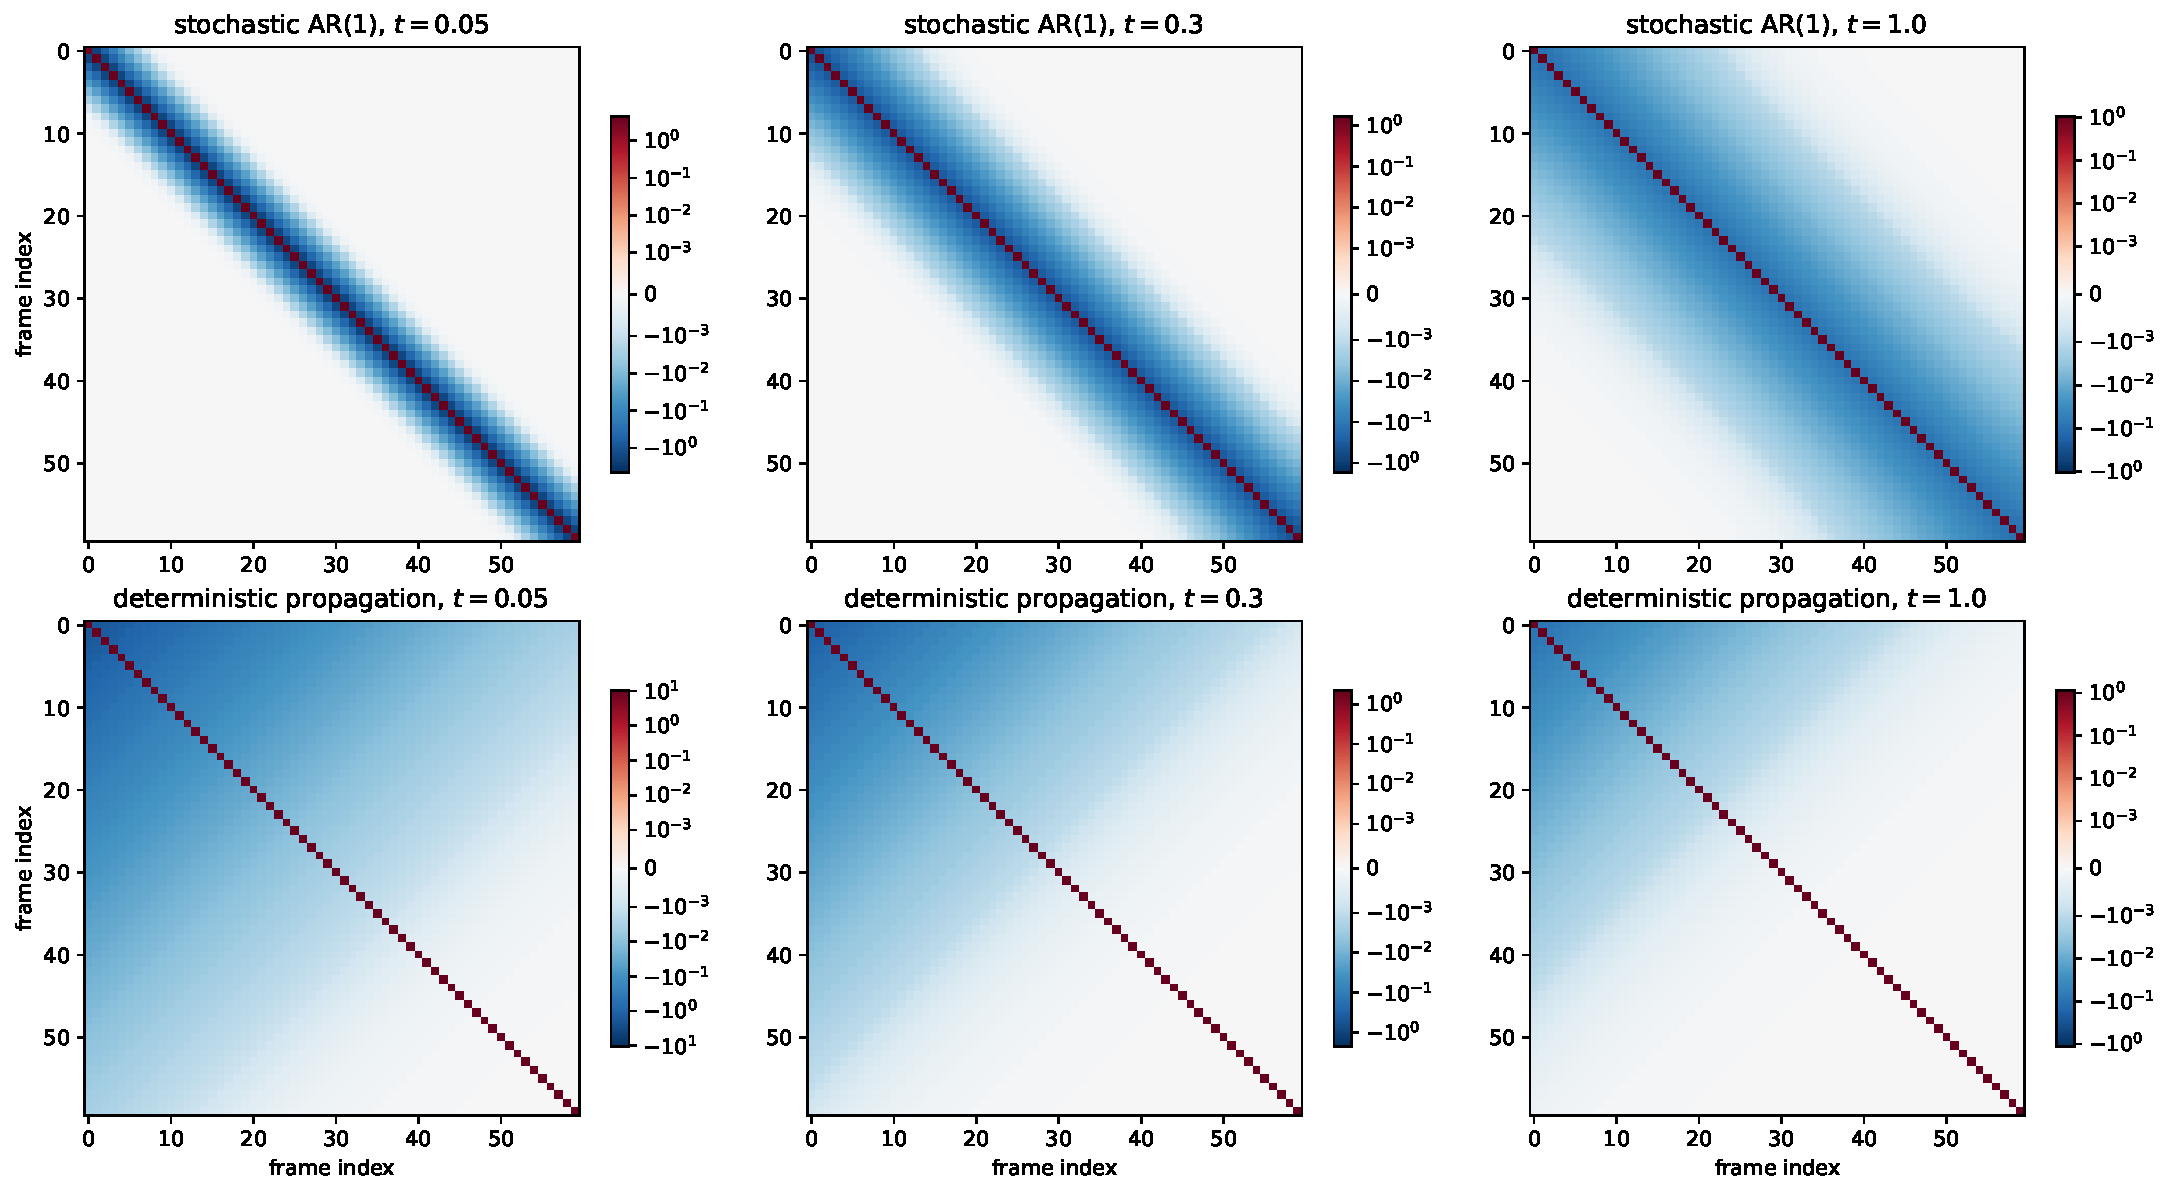
\includegraphics[width=.92\textwidth]{figures/fig09_deterministic_vs_stochastic_precision.pdf}
\caption{Deterministic versus stochastic benchmark. The deterministic model produces a diagonal-minus-rank-one noisy inverse, which is globally dense.}
\end{figure}

\section{First non-Gaussian extension}

A natural non-Gaussian chain is
\begin{equation}
 a_{k+1}=\alpha a_k+\varepsilon_k,
 \qquad \varepsilon_k\sim f,
\end{equation}
with known characteristic function $\widehat f(q)=\E[e^{iq\varepsilon_0}]$. Writing
\begin{equation}
 a_k=\alpha^ka_0+\sum_{\ell=0}^{k-1}\alpha^{k-1-\ell}\varepsilon_\ell,
\end{equation}
one finds the exact clean characteristic function
\begin{equation}
 \Phi_0(\xi)=\phi_0(L_0(\xi))\prod_{\ell=0}^{K-1}\widehat f(L_{\ell+1}(\xi)),
\end{equation}
where the $L_\ell$ are explicit tail linear forms. After OU noising,
\begin{equation}
 \Phi_t(\xi)=e^{-\frac{\Delta_t}{2}\|\xi\|^2}\Phi_0(e^{-t}\xi).
\end{equation}
So the Fourier-side formulation is exact for any kernel with known transform.

The strongest first extension is the \textbf{Laplace innovation model},
\begin{equation}
 f(u)=\frac{1}{2b}e^{-|u|/b},
 \qquad \widehat f(q)=\frac{1}{1+b^2q^2}.
\end{equation}
It is non-Gaussian, finite-variance, and has the Gaussian benchmark as its small-frequency tangent because
\begin{equation}
 \log\widehat f(q)=-b^2q^2+O(q^4).
\end{equation}
The object replacing the constant precision matrix is the score Hessian
\begin{equation}
 \mathcal H_t(\mathbf x)=-\nabla^2\log p_t(\mathbf x),
\end{equation}
which becomes $x$-dependent in the non-Gaussian regime.

\section{Takeaways}

\begin{enumerate}[label=(\arabic*),leftmargin=1cm]
\item The clean local Markov structure lives in the precision matrix, not in the covariance.
\item Diffusion does not merely weaken locality; it first delocalizes it and only later erases it.
\item The intermediate regime is quantitatively captured by band mass, effective bandwidth, interaction range, score-component correlations, and posterior-mean gain.
\item The deterministic benchmark shows that global score couplings can come from propagated latent uncertainty even without innovation randomness.
\item The Laplace chain is the best first non-Gaussian extension because it keeps a simple Fourier representation while genuinely breaking Gaussian affine structure.
\end{enumerate}

\begin{thebibliography}{99}

\bibitem{draftar1}
G.~Mantovani and M.~Lomel\'e.
\newblock \emph{Joint Score of a Diffusion Model Applied to an AR(1) Sequence: A Self-Contained Derivation}.
\newblock MSc thesis notes, Bocconi University, 2025--2026.

\bibitem{structure}
G.~Mantovani and M.~Lomel\'e.
\newblock \emph{The Structure of $\Sigma_t$ and $\Sigma_t^{-1}$ in the AR(1) Diffusion Model: Explicit Inversion, Spectral Decomposition, and Numerical Study}.
\newblock MSc thesis notes, Bocconi University, March 2026.

\bibitem{anatomy}
G.~Mantovani and M.~Lomel\'e.
\newblock \emph{The Anatomy of $\Sigma_t$ and $\Sigma_t^{-1}$: How Diffusion Noise Reshapes the Score of an AR(1) Sequence}.
\newblock MSc thesis notes, Bocconi University, March 2026.

\bibitem{companion}
G.~Mantovani and M.~Lomel\'e.
\newblock \emph{Mathematical Companion: Deep-Dive Explanations for the $\Sigma_t$ Analysis}.
\newblock MSc thesis notes, Bocconi University, March 2026.

\bibitem{mezardnotes}
M.~M\'ezard.
\newblock \emph{Generative Diffusion Updated Notes}.
\newblock Lecture notes, December 2025.

\bibitem{biroli2023}
G.~Biroli and M.~M\'ezard.
\newblock Generative diffusion in very large dimensions.
\newblock \emph{arXiv preprint arXiv:2306.03518}, 2023.

\bibitem{meetingtranscript}
G.~Mantovani, M.~Lomel\'e, M.~M\'ezard, and J.~Garnier-Brun.
\newblock \emph{Meeting transcript on the AR(1) diffusion benchmark and next research directions}.
\newblock Working transcript, March 2026.

\end{thebibliography}


\end{document}
